\documentclass[11pt,a4paper]{ivoa}
\input tthdefs
\input gitmeta
\usepackage[textsize=small,textwidth=3.8cm,backgroundcolor=yellow]{todonotes}
\newcommand{\subsubsubsection}[1]{\paragraph{#1}\mbox{}\\}
\setcounter{secnumdepth}{4}
\setcounter{tocdepth}{4}

\title{Authentication in the Virtual Observatory}

% see ivoatexDoc for what group names to use here; use \ivoagroup[IG] for
% interest groups.
\ivoagroup{Distributed Services and Protocols}

\author{Mark Taylor}
\author{Sara Bertocco}
\author{Patrick Dowler}
\author{Brian Major}
\author{Jesus Salgado}
\author{James Tocknell}
\author{Adrian Damian}
\author{Russ Allbery}

\editor{Mark Taylor}

% \previousversion[????URL????]{????Concise Document Label????}
\previousversion{This is the first public release}

\newcommand{\rfc}[1]{RFC\,#1}
\newcommand{\header}[1]{{\tt #1}}

\begin{document}

\begin{abstract}
This document explains how
VO services can manage the authentication process for
interoperability with clients, especially non-browser clients.
Particularly, this document
describes how services advertise their
support of specific authentication schemes and how
clients can discover and use this information to access protected
resources.
\end{abstract}


% \section*{Acknowledgments}


\section*{Conformance-related definitions}

The words ``MUST'', ``SHALL'', ``SHOULD'', ``MAY'', ``RECOMMENDED'', and
``OPTIONAL'' (in upper or lower case) used in this document are to be
interpreted as described in IETF standard RFC2119 \citep{std:RFC2119}.

The \emph{Virtual Observatory (VO)} is a
general term for a collection of federated resources that can be used
to conduct astronomical research, education, and outreach.
The \href{https://www.ivoa.net}{International
Virtual Observatory Alliance (IVOA)} is a global
collaboration of separately funded projects to develop standards and
infrastructure that enable VO applications.


\section{Introduction}\label{sec:intro}

Historically many services in the VO have operated primarily or
entirely in anonymous mode.
However authentication and associated authorization
are becoming increasingly necessary in the VO,
for instance to manage data rights and as an operational necessity for
auditing and limiting service usage in the era of science platforms.
% Some way to manage authentication for VO services is therefore necessary
% but not covered in all contexts by existing industry-standard machinery.

Where the client is browser-based
a service can often integrate information about the authentication
methods required with the web page or web application through which
it is accessed.

But a desktop VO client such as Aladin, TOPCAT or Python
typically interacts with VO services differently, in one of two
ways:
\begin{enumerate}
\item Searches the registry for a service, then makes VO-compliant
      requests to that service (e.g.\ TAP)
\item Is presented with a URL, then retrieves the data from that URL
      (e.g.\ DataLink)
\end{enumerate}
In the first, TAP-like, case additional information is available to the
client in the form of the Registry record for the service in question,
as defined by VOResource \citep{2008ivoa.spec.0222P}
and its service-specific extensions.
This could in principle contain metadata describing the authentication
method along with any required ancillary information such as
login endpoints.
Even if only the TAP service URL is available
(for instance because the user has typed it in rather than acquired it
from a Registry search) the VOSI Capabilities endpoint can be reliably
located ({\tt /capabilities} is a sibling of {\tt /sync} in TAP),
so that relevant VOResource information could be retrieved from the VOSI
Capabilities document supplied by the service.

However in the second, DataLink-like, case
there is no information about where to find a corresponding
registry record or VOSI document,
or even a guarantee or likelihood that such a record exists.
The URL in question may not even have come from a DataLink query,
it could simply be a pointer to a protected resource like a
FITS file or VOTable in a secured filestore.
Such a URL may have been acquired from a VO query in the application
wishing to dereference it, in which case some authentication context
may be available,
but it may equally be read from a VOTable transmitted by SAMP
or saved in an earlier session, or obtained from an unrelated application;
in other words the application requiring the resource at a URL may
have no information about the VO service which produced that URL.
Then the only opportunity to acquire information about how to authenticate
is by examining the URL itself, or by HTTP communications with that URL,
where authentication requirements are reported using the standard
challenge/response framework reviewed in Section~\ref{sec:challenge-response}.

An authentication method like HTTP Basic (\rfc{7617})
can be used straightforwardly in this scenario,
since all negotiation involving user credentials and permits ---
request and supply of username and password ---
is done directly
over the HTTP connection from which the resource is requested.

More modern/secure/flexible authentication methods however tend to
rely on additional prior interaction with other endpoints
distinct from the resource location itself.
Industry standard mechanisms enabling clients to discover
these interaction requirements
in absence of out-of-band information tend to be lacking or non-obvious.
This document explains in Section~\ref{sec:authschemes}
how services can be configured to permit such discovery.
In the case of Bearer Tokens this is done by prescribing a profile
of existing industry standards to enable it (Section~\ref{sec:ivoa-bearer}),
and in the case of cookie and certificate use it is done by
defining a non-standard authentication challenge by which
services can supply the missing information (Section~\ref{sec:voschemes}).
It also describes (Section~\ref{sec:cr-use}) how to discover the
authentication requirements for VO services, and
some arrangements for working with optional authentication.

The intent of this document is not to define new authentication
mechanisms parallel to pre-existing standards, but to provide
missing components that facilitate use of such existing standards
from certain VO contexts, especially by non-browser clients.
Authenticated services in the VO are not expected to change their
authentication frameworks to any ``VO-sanctioned'' technology,
but by implementing the proposals here they can become usable
in a broader range of scenarios.
VO services however are not required to use any of the
mechanisms proposed in this document; if they can establish the
client interoperability they require using other mechanisms, or
a combination of VO and other mechanisms, they are free to do so.

Given that, as explained above,
the VOResource record can only be discovered in some (TAP-like)
and not other (DataLink-like) authentication scenarios,
it is no longer recommended to base discovery of authentication methods
on the {\tt securityMethod} element
defined by VOResource, as described by SSO 2.0.
Instead, the challenge/response-based approach described here
should be used for both TAP-like and DataLink-like scenarios.

\subsection{Role within the VO Architecture}

\begin{figure}
\centering

% As of ivoatex 1.2, the architecture diagram is generated by ivoatex in
% SVG; copy ivoatex/archdiag-full.xml to role_diagram.xml and throw out
% all lines not relevant to your standard.
% Notes don't generally need this.  If you don't copy role_diagram.xml,
% you must remove role_diagram.pdf from SOURCES in the Makefile.

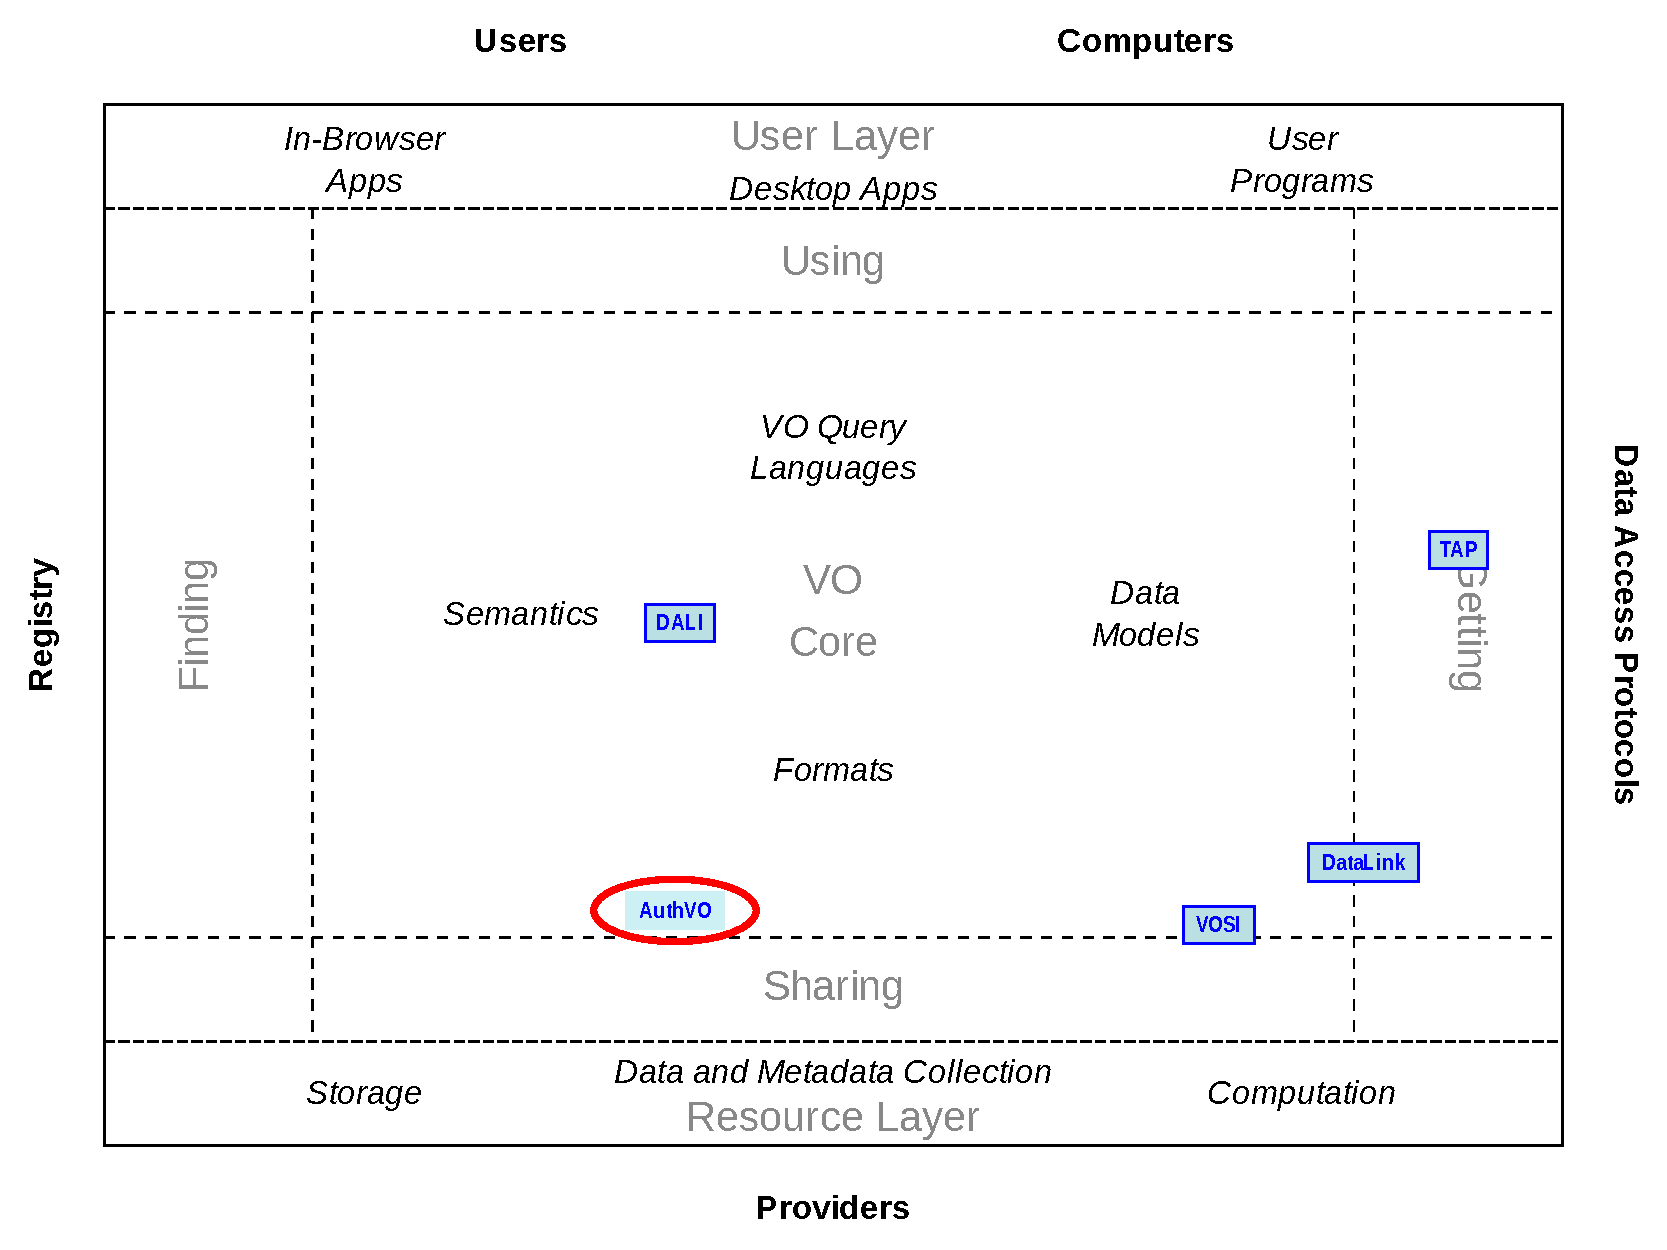
\includegraphics[width=0.9\textwidth]{role_diagram.pdf}
\caption{Architecture diagram for this document}
\label{fig:archdiag}
\end{figure}

Fig.~\ref{fig:archdiag} shows the role this document plays within the
IVOA architecture \citep{2021ivoa.spec.1101D}.

AuthVO provides a way to advertise authentication methods
associated with existing VO services.
For services like TAP \citep{2019ivoa.spec.0927D}
that comply with VOSI \citep{2017ivoa.spec.0524G} to
offer service description documents at locations
defined by DALI \citep{2017ivoa.spec.0517D},
clients can discover these methods
using an up-front query to the VOSI capabilities endpoint.
For non-VOSI services such as DataLink \citep{2015ivoa.spec.0617D}
such discovery is done reactively.


\subsection{Terminology}

The following terms are used with specific meanings in this document:

\begin{description}
\item[protected]
      A service or resource that can only be accessed by authenticated users,
      or will allow greater levels of access to authenticated users over
      anonymous users
\item[permit]
      Information that a client can supply with an HTTP request to
      prove its authenticated identity;
      may for instance be a token, cookie or certificate
\item[credentials]
      Secret information known to a user, such as a username and password,
      that can be used to acquire a {\em permit}
\item[domain]
      A set of HTTP endpoints sharing the same authentication arrangements;
      the same {\em permit\/} is applicable to all members of the same domain
      and should not be presented to endpoints outside that domain
\item[challenge]
      A structured invitation to authenticate using
      a particular {\em permit\/} type,
      presented within a \header{WWW-Authenticate} header
\item[authentication scheme]
      A particular type of {\em challenge\/} with its own rules and syntax
\end{description}
The terms {\em challenge\/} and {\em authentication scheme} are
defined by \rfc{9110}
and explained further in Section~\ref{sec:challenge-response-details}.


\section{Challenge and Response}
\label{sec:challenge-response}

The standard way to negotiate authentication over HTTP is using
authentication challenges supplied in HTTP responses.
This challenge/response framework forms the basis for the
authentication behaviour recommended by this document.

\subsection{Challenge/Response Framework}
\label{sec:challenge-response-details}

The basics of authentication over HTTP can be found in
section 11 of \rfc{9110} \citep{std:RFC9110};
that document obsoletes \rfc{7235} \citep{std:RFC7235}
which presented an earlier version of this protocol.
More detail can be found in those documents, but for convenience
the basics are outlined here:
% 401, 403, WWW-Authenticate, maybe Authorization.
\begin{itemize}
  \item An HTTP response may include one or more
        \header{WWW-Authenticate} headers
        to indicate that authentication is possible.
        The content of these headers is one or more {\em challenges},
        each describing how the client can authenticate according
        to a named {\em authentication scheme}.
  \item A 401 (Unauthorized) response MUST include at least one such challenge
  \item Other (e.g. 200 OK, 403 Forbidden) responses
        MAY include such challenges
  \item The client may use the challenge information to decide how
        to authenticate itself to the server in subsequent requests.
        This can be done by supplying the \header{Authorization} header
        with scheme-specific content.
        In case of multiple challenges, the client is free to choose one.
  \item The form of a challenge is:\\
        \verb|   <auth-scheme-name> [<scheme-specific-parameters>]|
  \item The form of the \header{WWW-Authenticate} header is:\\
        \verb|   WWW-Authenticate: <challenge> [<challenge> ...]|
\end{itemize}

The details of a number of these authentication schemes
(\verb|<auth-scheme-name>| strings and their
associated parameters and semantics)
are defined in IETF documents, for instance
``{\tt basic}'' (\rfc{7617} \citet{std:RFC7617}),
``{\tt digest}'' (\rfc{7616} \citet{std:RFC7616})
and
``{\tt bearer}'' (\rfc{6750} \citet{std:RFC6750}).
\rfc{9110} section 11.1 says
``New and existing authentication schemes are
  specified independently and ought to be registered''
  (\href{https://www.iana.org/assignments/http-authschemes}{with IANA}),
but it does not say that they MUST be so registered.



\subsection{Authentication Schemes in the VO}

Where one of the standard authentication schemes is
suitable for use by a particular VO service and its clients,
it should be used.
For instance Basic (\rfc{7617}) or Digest (\rfc{7616}) authentication
provide all required
information about the authentication procedure within the headers,
since the client simply supplies
(somewhat obscured) username and password
to the target service in subsequent requests.
If these schemes are used it is highly recommended
to require a TLS connection (HTTPS not HTTP) to avoid interception of
the credentials.

Services using OAuth2 generally make use of the Bearer scheme.
In this case the challenged client supplies a {\em bearer token}
in subsequent requests,
but a usual \verb|Bearer| challenge provides no information about how to
acquire such a token, which means it is not suitable for clients lacking
prior knowledge about the target service, as described in
Section~\ref{sec:intro}. To support those clients, this document profiles the
standard \verb|Bearer| scheme (Section~\ref{sec:ivoa-bearer}), whose challenge
carries a pointer to a Protected Resource Metadata document (\rfc{9728}~\citep{std:RFC9728}) from
which the client can discover the authorization server, confirm from that
server's own metadata that it issues tokens for this resource, and obtain a
token, preferably one whose audience is restricted to the resource.

Other methods of authentication over HTTP also exist
and are used by VO services,
for instance use of cookies and of X.509 certificates.
In standard usage these do not present \header{WWW-Authenticate} challenges,
and again prior knowledge about the service
(how to acquire a suitable cookie or certificate)
is required by the client to use them.
This document defines in \ref{sec:voschemes}
some VO-specific authentication schemes
that solve these problems by supplying the missing information to
clients in scheme-specific challenge parameters.

\section{Authentication Schemes}\label{sec:authschemes}

The authentication schemes defined in this section
generally define:
\begin{enumerate}
  \item How clients are to present a permit in future requests
        to a service --- this is defined by the identity of the scheme
  \item How they are to acquire such a permit ---
        this is communicated by the scheme-specific parameters
  \item The {\em authentication domain\/}, i.e.\ at which endpoints the permit
        should be used --- this is determined in a scheme-specific way
\end{enumerate}

The last of these, the rule about the set of endpoints within which
an acquired permit is valid, needs careful consideration.
The permit is confidential information and so must not be leaked to services
outside the domain,
but existing permits should be used for all endpoints within their domain
so that the user is not made to present their credentials multiple times
unnecessarily.
The client may also be managing multiple permits
for multiple different domains at once.
So the permit must be delivered with sufficient
implicit or explicit domain
information for the client to tell for each subsequent request
whether that permit should be presented,
i.e.\ whether it falls within that permit's domain.
The nature and form of this domain information is scheme-specific.



\subsection{VO-Specific Scheme Definitions}\label{sec:voschemes}

This section defines some custom Authentication Schemes
for use in \header{WWW-Authenticate} challenges,
intended for use within the VO.
The purpose of these is to advertise usage information to VO clients
about a standard authentication method in use
(currently, cookies or certificates).

% mboxes required to stop TtL barfing on underscores
\subsubsection{\mbox{\tt ivoa\_cookie}}\label{sec:ivoa-cookie}

The \verb|ivoa_cookie| authentication scheme indicates that the service
will accept cookies as authentication permits,
and describes how to acquire such cookies.

\begin{description}
  \item[Scheme name:] \verb|ivoa_cookie|
  \item[Parameters:] (see Section~\ref{sec:common-params})
  \begin{itemize}
    \item \verb|access_url| (required) ---
          indicates where to get the cookie
    \item \verb|standard_id| (required) ---
          indicates how to authenticate at \verb|access_url|
  \end{itemize}
  \item[Login response:] \header{Set-Cookie} header
  \item[Domain:] As defined by \rfc{6265}
\end{description}

Cookies are text strings received in the {\tt Set-Cookie}
response header of some HTTP exchange,
and presented via the {\tt Cookie} request header of subsequent
requests to the same service.
This procedure is defined in \rfc{6265} \citep{std:RFC6265}.
A parallel mechanism using the {\tt Set-Cookie2} and {\tt Cookie2}
headers was also defined by an earlier version of the cookie protocol
defined in \rfc{2965} \citep{std:RFC2965},
but this is now deprecated and rarely used.

To use this scheme, the client must present a username and password
to the endpoint given by the \verb|access_url| parameter,
in the form defined by the \verb|standard_id| parameter
(see Section~\ref{sec:common-params}).
If authentication is successful, a 200 OK response must be returned
including a \header{Set-Cookie} header containing one or more cookies
suitable as an authentication permit.
If authentication fails, a 401 or 403 response should be returned.
Once in possession of the returned cookie or cookies,
the client can present them in a \header{Cookie} header as defined
by \rfc{6265} for subsequent requests to protected resources.
If multiple cookies were received, they should all be presented.

Cookies come with an associated domain, defined by the content
of the \header{Set-Cookie} header in conjunction with \rfc{6265},
so compliant cookie-handling
libraries are able to determine the domain for a given cookie.

There is an example in Section~\ref{sec:cookie-example}.


\subsubsection{\mbox{\tt ivoa\_x509}}\label{sec:ivoa-x509}

The \verb|ivoa_x509| authentication scheme indicates that the service
will accept X.509 client certificates as authentication permits,
and optionally describes how to acquire a suitable certificate.

The standard usage model for X.509 certificates is that 
a person or organisation obtains a certificate from a
Certification Authority (CA) once its identification has
been verified by a Registration Authority.

A client in posession of a client certificate can then use it to
sign TLS (HTTPS) connections, and the service can examine the signature
to authenticate the identity of the client.
Such authentication will succeed if the service trusts the signing CA.

\begin{description}
  \item[Scheme name:] \verb|ivoa_x509|
  \item[Parameters:] (see Section~\ref{sec:common-params})
  \begin{itemize}
    \item \verb|access_url| (optional) ---
          indicates where to get a suitable certificate
    \item \verb|standard_id| (required if \verb|access_url| is present) ---
          indicates how to authenticate at \verb|access_url|
  \end{itemize}
  \item[Login response (if used):] PEM-encoded X.509 certificate chain
                                   including private key
  \item[Domain:] Origin of challenge URL
\end{description}

The \verb|ivoa_x509| challenge exists in two forms:
with and without the \verb|access_url|/\verb|standard_id| parameter pair.
These optional parameters advise the client how to obtain a certificate
for use within the domain of the challenge if it does not already have one.

For either form of the challenge,
if the client is in possession of a certificate
signed by a CA it expects the service to trust, it may use it to
sign requests to protected resources within the domain of the challenge.

If the client does not hold any such certificate,
and the \verb|access_url|/\verb|standard_id| pair is present,
it may obtain one by presenting credentials
to the endpoint given by the \verb|access_url| parameter,
in the form defined by the \verb|standard_id| parameter
(see Section~\ref{sec:common-params}).
If authentication is successful, a 200 OK response must be returned
whose body is an X.509 certificate chain including its private key,
in PEM format.  The \header{Content-Type} header of this response
should be ``{\tt application/x-pem-file}''.
If authentication fails, a 401 or 403 response should be returned.
Once in possession of the returned certificate,
the client can use it to sign subsequent requests to protected resources.
Certificates obtained in this way may not be usable in all X.509 contexts
(i.e. may not be signed by a widely trusted CA),
but should be usable within the domain of the current challenge.

Since client certificates achieve authentication by signing requests
using public key cryptography, they cannot be stolen by third parties,
so there are no security issues associated with attempting to use them
to access services outside of the intended authentication domain.
However using them for inapplicable services is inefficient and clumsy
so some rule for domain determination is desirable.
The authentication domain of a certificate acquired using this scheme is
considered to be the {\em Origin\/} of the URL from which
the challenge was received.
Origin is defined by section 4.3.1 of \rfc{9110}
and is a normalised triple of URI scheme, hostname, and port.

There is an example in Section~\ref{sec:x509-example}.

\subsubsection{Common Challenge Parameters for VO-Specific Schemes}
\label{sec:common-params}

The VO-specific authentication schemes described in
Section~\ref{sec:voschemes}
rely on a stage where the user ``logs in'' by exchanging
credentials (a username and password) for a permit.
This section defines common challenge parameters that
tell the client exactly where and how to present these credentials.

\begin{description}
\item[{\tt access\_url}:]
  The \verb|access_url| parameter reports where to log in:
  the value is the endpoint at which
  exchange of user credentials for a permit
  takes place.
%
\item[{\tt standard\_id}:]
  The \verb|standard_id| parameter explains how to log in:
  it defines the protocol for exchanging user credentials
  for a permit.
  Username and password are supplied in the HTTP request as described below,
  and the response returns a scheme-specific permit.
  Currently defined values are:
  \begin{description}
    \item[{\tt ivo://ivoa.net/sso\#BasicAA}]
          The Basic Authentication scheme defined by \rfc{7617} is used to
          authenticate.
          It is STRONGLY RECOMMENDED to use this over HTTPS not HTTP,
          since the username and password are transmitted without encryption.
    \item[{\tt ivo://ivoa.net/sso\#tls-with-password}]
          The username and password are presented using a POST request
          over an HTTPS connection.
          These items are passed as the values of parameters
          ``{\tt username}'' and ``{\tt password}'' respectively,
          transmitted in {\tt application/x-www-form-urlencoded} format.
  \end{description}
\end{description}


\subsection{Bearer Tokens}\label{sec:ivoa-bearer}

VO services that require OAuth~2.0 (\rfc{6749}~\citep{std:RFC6749}) access tokens use the standard
\verb|Bearer| authentication scheme (\rfc{6750}) in their
\header{WWW-Authenticate} challenges; this document does not define a
VO-specific scheme for them. What it adds --- crucially for clients with no
prior knowledge of the service --- is a profile that tells the client how to
discover the authorization server and how to confirm that it is safe to log in
and present a token to this particular resource. The profile combines the
\verb|Bearer| scheme with OAuth~2.0 Protected Resource Metadata (\rfc{9728})
and Authorization Server Metadata (\rfc{8414}~\citep{std:RFC8414}).

The scheme supports headless clients (e.g.\ command-line tools or scripts)
through the Device Authorization Grant (\rfc{8628}~\citep{std:RFC8628}), token expiry and renewal
through refresh tokens, and zero-touch onboarding through Dynamic Client
Registration (\rfc{7591}~\citep{std:RFC7591}); it integrates with standard OAuth2/OIDC
infrastructures.

A bare \verb|Bearer| challenge (\rfc{6750}) gives the client no way to discover
where to obtain a token. Under this profile the challenge instead carries a
\verb|resource_metadata| parameter (\rfc{9728}) pointing at the
\emph{Protected Resource Metadata} (PRM) document of the resource: a small JSON
document, published by the protected resource itself at its \rfc{9728}
well-known location, that names the authorization server(s) for this resource.
Because a malicious resource can name any authorization server in its PRM,
the client does not accept that claim on its own. It confirms it against the
authorization server's own metadata, which lists the resources the server
issues tokens for, \emph{before} the user is asked to log in or any token is
sent (Section~\ref{sec:ivoa-bearer-flow}).

\begin{description}
  \item[Scheme name:] \verb|Bearer| (\rfc{6750})
  \item[Parameters:] \mbox{}
  \begin{itemize}
    \item \verb|resource_metadata| (required) --- the URL of the Protected
          Resource Metadata document (\rfc{9728}) of this resource, at the
          well-known location defined in \rfc{9728} section 3.
          It MUST be served over HTTPS, and the document it points to is
          \emph{untrusted} until the checks of
          Section~\ref{sec:ivoa-bearer-flow} have passed.
    \item \verb|error| (optional) --- one of the error codes defined by
          \rfc{6750} section 3.1: \verb|invalid_request|,
          \verb|invalid_token| or \verb|insufficient_scope|. It is omitted
          when the request carried no token.
    \item \verb|error_description| (optional) --- a human-readable explanation
          of the error condition.
  \end{itemize}
  \item[Domain:] the resource identifier named in the PRM document, together
        with the URLs below it (Section~\ref{sec:ivoa-bearer-as}); where the
        token is audience-bound, its audience is that resource
        (see Section~\ref{sec:ivoa-bearer-flow}).
\end{description}

When a protected resource is accessed without any token, the service
responds with a 401 that carries \emph{only the pointer}, never the descriptor
itself. Since the request carried no authentication information, the challenge
carries no error information either (\rfc{6750} section 3.1):

{\small
\begin{verbatim}
HTTP/1.1 401 Unauthorized
WWW-Authenticate: Bearer
  resource_metadata=
    "https://data.example.org/.well-known/oauth-protected-resource/vo"
\end{verbatim}
}

When the request carried a token that is invalid or has expired, the
challenge adds the \verb|error| parameter, together with the same pointer so
that the client can obtain a new token:

{\small
\begin{verbatim}
HTTP/1.1 401 Unauthorized
WWW-Authenticate: Bearer
  resource_metadata=
    "https://data.example.org/.well-known/oauth-protected-resource/vo",
  error="invalid_token",
  error_description="The access token expired"
\end{verbatim}
}

The \verb|resource_metadata| URL MUST resolve to a Protected Resource Metadata
document conforming to \rfc{9728}, published by the protected resource. Its key
members are:

\begin{itemize}
  \item \verb|resource| --- the identifier of the protected resource. It MUST
        cover the URL whose request produced the challenge, as defined in
        Section~\ref{sec:ivoa-bearer-as}.
  \item \verb|authorization_servers| --- one or more issuer identifiers of the
        authorization servers for this resource. The client trusts an entry
        only after confirming the resource against that server's own metadata
        (Section~\ref{sec:ivoa-bearer-flow}).
  \item \verb|scopes_supported| --- the OAuth scopes the resource understands.
  \item \verb|bearer_methods_supported| --- how the token may be presented;
        \verb|header| denotes the \header{Authorization: Bearer} form.
\end{itemize}

A minimal PRM document looks like:

\begin{verbatim}
{
  "resource": "https://data.example.org/vo",
  "authorization_servers": ["https://iam.example.org/"],
  "scopes_supported": ["read"],
  "bearer_methods_supported": ["header"]
}
\end{verbatim}

From the issuer named in \verb|authorization_servers|, the client retrieves the
Authorization Server Metadata (\rfc{8414}), which provides the list of
protected resources and the endpoints the flow needs:

\begin{itemize}
  \item \verb|protected_resources| --- the resource identifiers this server
        issues tokens for (\rfc{9728} section 4); required by this profile,
        see Section~\ref{sec:ivoa-bearer-as}.
  \item \verb|token_endpoint| --- to obtain access and refresh tokens.
  \item \verb|device_authorization_endpoint| --- to start a device-code login
        for headless clients (\rfc{8628}).
  \item \verb|registration_endpoint| --- for Dynamic Client Registration
        (\rfc{7591}).
  \item \verb|authorization_endpoint| --- to start a browser-based login.
  \item \verb|grant_types_supported|, \verb|scopes_supported| --- the supported
        grant types and scopes.
\end{itemize}

Only the three \rfc{6750} codes above appear in the \verb|Bearer| challenge
itself. The other errors a client following this profile may meet are
returned by the authorization server's endpoints during the flow of
Section~\ref{sec:ivoa-bearer-flow}. Table~\ref{table:oAuthCodes} lists the
common ones, where the client meets them, and where each is defined.
\begin{table}[]
\centering
\small
\begin{tabular}{lll}
\textbf{Error code} & \textbf{Where the client meets it} & \textbf{Defined in} \\
\hline
{\tt invalid\_request} & Bearer challenge, token endpoint & \rfc{6750}, \rfc{6749} \\
{\tt invalid\_token} & Bearer challenge (401) & \rfc{6750} \S3.1 \\
{\tt insufficient\_scope} & Bearer challenge (403) & \rfc{6750} \S3.1 \\
\hline
{\tt invalid\_client} & token endpoint & \rfc{6749} \S5.2 \\
{\tt invalid\_grant} & token endpoint (e.g.\ bad refresh token) & \rfc{6749} \S5.2 \\
{\tt unauthorized\_client} & token endpoint & \rfc{6749} \S5.2 \\
{\tt invalid\_scope} & token endpoint & \rfc{6749} \S5.2 \\
{\tt invalid\_target} & token endpoint ({\tt resource} rejected) & \rfc{8707} \S2 \\
\hline
{\tt authorization\_pending} & device grant: keep polling & \rfc{8628} \S3.5 \\
{\tt slow\_down} & device grant: poll less often & \rfc{8628} \S3.5 \\
{\tt access\_denied} & device grant: user refused & \rfc{8628} \S3.5 \\
{\tt expired\_token} & device grant: code expired, restart & \rfc{8628} \S3.5 \\
\end{tabular}
\caption{OAuth~2.0 error codes a client may meet in this profile}
\label{table:oAuthCodes}
\end{table}

If a client does not already have a \verb|client_id|, it MUST obtain one via
Dynamic Client Registration as described in \rfc{7591}. The URL of the
registration endpoint is given in the \verb|registration_endpoint| field of
the discovery document. Clients MUST NOT assume this value and MUST always
obtain it from the advertised discovery metadata. See
\ref{sec:ivoa-bearer-flow} for flow and security details.

\subsubsection{Authorization Server Requirements}\label{sec:ivoa-bearer-as}

Authorization servers used with this profile MUST publish Authorization Server
Metadata (\rfc{8414}) that includes the \verb|protected_resources| member
(\rfc{9728} section 4), listing the identifiers of the protected resources for
which they issue tokens. This member is optional in \rfc{9728}; it is
mandatory here because it is what allows a client to distinguish a genuine
resource from one that merely names the authorization server in its PRM. If
the same metadata is also published as an OpenID Connect Discovery document,
the member SHOULD be included there as well.

A resource identifier, whether in \verb|protected_resources| or in the
\verb|resource| member of a PRM document, \emph{covers} a URL if the URL is
equal to it, or has the same scheme, host and port and a path that extends it
at a path-segment boundary. For instance, the identifier
{\tt https://data.example.org/vo}:
\begin{itemize}
  \item covers {\tt https://data.example.org/vo/tap/async/123};
  \item does not cover {\tt https://data.example.org/vocab}.
\end{itemize}
This relaxes the exact match required by \rfc{9728} section 3.3,
so that one identifier can govern a whole service whose endpoints
have variable paths. A client that applies \rfc{9728} section 3.3 to the
letter will therefore reject such a PRM when the challenge came from a URL
below the identifier: this profile needs clients that implement the coverage
rule above.

Authorization servers SHOULD reject a token request whose \verb|resource|
parameter (\rfc{8707}~\citep{std:RFC8707}) is not covered by an entry of their
\verb|protected_resources|, with the \verb|invalid_target| error defined in
\rfc{8707} section 2, and SHOULD issue tokens whose audience is restricted
to the requested resource (Section~\ref{sec:ivoa-bearer-flow}, Step~5).

{\itshape Note (non-normative): audience restriction in practice.
Not all authorization servers implement these recommendations. For instance,
INDIGO IAM accepts its own {\tt aud} and {\tt audience} request parameters
and, from version 1.12, also the \rfc{8707} {\tt resource} parameter, and
places the requested value in the {\tt aud} claim of the access token; but it
does not compare the requested value with a list of allowed resources, so an
unlisted resource does not cause {\tt invalid\_target}. Version 1.10 ignores
{\tt resource} altogether: in the reference implementation
\citep{authvo-clients} it issued equivalent tokens, without an {\tt aud}
claim, for a listed, an unlisted and an absent {\tt resource}. With such a
server, the resource check of Step~3 is the only protection against a service
that merely names the authorization server in its PRM. Where an
audience-restricted token can still be obtained, it limits the replay of a
leaked token at other listed resources.}

{\itshape Note (non-normative): emulating \verb|protected_resources|.
Some authorization server products do not yet publish the
\verb|protected_resources| member. Until they do, operators can add it with
the reverse proxy that fronts the authorization server: the proxy retrieves
the server's live metadata, adds the member from local configuration, and
returns the documents at their usual URLs with all other members unchanged.
Where the product publishes only an OpenID Connect Discovery document and no
\rfc{8414} document (INDIGO IAM is an example), the proxy also serves an
\rfc{8414} document at {\tt /.well-known/oauth-authorization-server},
derived from the OpenID Connect one with the same {\tt issuer} and endpoints,
since clients use the \rfc{8414} document for the resource check. Clients cannot distinguish this
from native support, and the proxy rule can be removed once the product
implements the member. The reference implementation \citep{authvo-clients}
demonstrates this with INDIGO IAM. An authorization server that publishes the
member neither natively nor in this way cannot be used with this profile:
clients will refuse it (Section~\ref{sec:ivoa-bearer-flow}, Step~3).}


\section{Challenge/Response Use in the VO}
\label{sec:cr-use}

\subsection{Authentication Modalities}
\label{sec:modalities}

VO services can behave in three different ways with respect to authentication:
\begin{description}
  \item[No authentication:]
       all access is anonymous
  \item[Mandatory authentication:]
       anonymous access is always rejected, but once authenticated,
       user requests may be successful (subject to authorization)
  \item[Optional authentication:]
       anonymous requests may succeed, but authentication is possible
       and service behaviour may differ for anonymous and authenticated access;
       for instance a TAP service may expose more tables or relax
       usage limits for authenticated users
\end{description}
% The first two cases are fairly straightforward to deal with,
% the last one is a bit more subtle.

The standard HTTP rules for authentication cover the cases of
no authentication and mandatory authentication:
if a client requests a resource for which it is not authenticated,
the response should return a 401 Unauthorized code with an associated
\header{WWW-Authenticate} challenge
(or possibly a 403 Forbidden, optionally with a challenge).

To cover all three cases,
including allowing clients to determine that authentication may be an
option before presenting a possibly lengthy query,
VOSI-compliant services should implement the following behaviour
for both GET and HEAD requests to their VOSI-capabilities endpoint:
\begin{itemize}
  \item No authentication:
        return 200
  \item Mandatory authentication:
        return 401/403 with one or more \header{WWW-Authenticate} challenges
  \item Optional authentication:
        return 200 with one or more \header{WWW-Authenticate} challenges
\end{itemize}
VO clients can then probe the capabilities endpoint using an HTTP HEAD
or GET request to find out whether an authentication attempt should be
required or offered to the user, prior to making queries on the service.

\subsection{Client Behaviour}

Given the rules in Section~\ref{sec:modalities},
client requests to potentially authenticated URLs should
fall into one of the following categories:
\begin{description}
\item[Anonymous]
      A client with no capability to authenticate operates in Anonymous mode.
      Any attempt to retrieve protected resources will fail.
\item[Reactive]
      An unauthenticated client requiring a
      resource simply requests it anonymously.
      If the request is successful
      (typically an HTTP 200 OK response, perhaps via some 3xx redirects),
      no authentication is attempted.
      However, if the response is a 401 or 403 accompanied by
      one or more supported challenges,
      the client chooses a challenge it is prepared to use,
      and negotiates challenge-specific authentication as described above.
      On successful authentication, the acquired permit is used to
      retrieve the resource, and is also cached alongside its domain
      for future use.
      In case of a 401 or 403 without any challenges supported by the client,
      or if authentication fails, retrieval of the resource fails.
\item[Proactive]
      Once a client has authenticated to a domain,
      it should accompany any subsequent request to a resource
      in the same domain
      with the permit that it has cached from that domain.
      In this way, the user is not required to present credentials
      multiple times for the same domain.
\item[Preemptive]
      When talking to a VOSI-compliant service that may provide
      optional authentication,
      the client should first probe the VOSI-Capabilities endpoint
      using a HEAD or GET request.
      In case of a 401 or 403 response
      it should require the user to authenticate
      using one of the presented challenges,
      cache the permit, and make subsequent requests
      to that service in Proactive mode;
      if that authentication fails then the service cannot be used.
      In case of a 200 response it should check the response for challenges;
      if a supported challenge is present it may give the user the
      option to authenticate, and if successful cache the permit and
      make subsequent requests in Proactive mode.
      If no challenges are present (no authentication),
      or if the user elects not to authenticate,
      or if optional authentication fails,
      it should make subsequent requests in Anonymous or Reactive mode.
\end{description}

When using a VOSI-compliant service like TAP,
an authentication-capable client should initially probe
the capabilities in {\em preemptive\/} mode.
For all other requests it should check whether the URL
belongs to any of the domains for which it has a cached permit,
and query in {\em reactive\/} or {\em proactive\/} mode accordingly.


\subsection{Authentication Confirmation: {\tt X-VO-Authenticated}}

The case of optional authentication presents the question
of how a client knows whether it is authenticated or not.
Since a service with optional authentication can return
a successful (200 OK) result to both an authenticated and unauthenticated
client,
the client cannot use the HTTP response code to determine whether
an authentication attempt has been successful.

It is therefore RECOMMENDED that services include the header
\header{X-VO-Authenticated}, with a value giving the client's
authenticated identity, in all responses to an authenticated client,
and especially in response to any intial authentication attempt.
Responses to unauthenticated clients MUST NOT contain this header.


\subsection{Compatibility with other VO Standards}

Section~\ref{sec:modalities} of this document
makes use of HEAD requests to the capabilities endpoint,
but VOSI 1.1 \citep{2017ivoa.spec.0524G}
only requires capabilities to support GET.
If a client finds that HEAD is not supported (405 Method Not Allowed)
it may assume that optional authentication is not in place.

Section~\ref{sec:modalities} also allows a GET or HEAD request
to the capabilities endpoint to result in a
401 Unauthorized or 403 Forbidden failure,
but VOSI 1.1 Section 2 and TAP 1.1 Section 2.2 both require
the capabilities endpoint to be accessible anonymously.

The SSO 2.0 recommendation \citep{2017ivoa.spec.0524T}
requires that protected services
record their authentication requirements via a
\xmlel{SecurityMethod} element in their VOResource record.
This document does not align with SSO 2.0,
and \xmlel{SecurityMethod} elements are no longer required or recommended.

A service implementing the behaviour described here may therefore
be forced into conflict with existing VO documents.
Future evolution of those documents may act to resolve this conflict.

\subsection{Limitations}

This document does not currently make explicit provision for
expiry of permits.
Use of an expired permit will probably look like an authentication
failure (401), so clients may simply try to re-authenticate in
such a case.
In some cases scheme-specific expiry information may be supplied with a permit.
Future versions of this document may tackle this in more detail.


\section{Examples}

This section contains examples of communications between clients
and authenticating services.
Client behaviour is represented using the
command-line HTTP client {\tt curl};
this means that the HTTP headers of the query
are not shown in the examples,
but they can be examined by repeating the curl invocations
with the {\tt --verbose} flag.
The ``{\tt -D -}'' flag causes response headers to be shown.
Some of the non-essential headers have been removed for the sake
of brevity, and some line-breaks imposed for readability.

\subsection{Reactive authentication with HTTP Basic Authentication}

% This example is based on the resource at
% http://www.g-vo.org:8080/getproduct/feros/data/f04031.fits.vot and
% http://www.g-vo.org:8080/getproduct/feros/data/f04031.fits

Request a resource anonymously:
{\footnotesize
\begin{verbatim}
% curl -D - https://example.org/data/release/table99.vot
HTTP/1.1 401 Unauthorized
WWW-Authenticate: Basic realm="Gormenghast"
Content-Type: text/plain

Please log in.
\end{verbatim}
}

\noindent
This gives a 401 Unauthorized response
with a standard Basic challenge (\rfc{7617}).
We therefore resubmit the query with a username and password:
{\footnotesize
\begin{verbatim}
% curl --user gertrude:xxxx -D - https://example.org/data/release/table99.vot
HTTP/1.1 200 OK
X-Vo-Authenticated: gertrude
Content-Type: application/x-votable+xml

<?xml version='1.0' encoding='utf-8'?>
<VOTABLE version="1.5" ...
...
</VOTABLE>
\end{verbatim}
}

\noindent
We can then use the same permit (encoded username and password)
preemptively for other resources within the same domain
(defined in this context by \rfc{7617} as locations in the same
directory or its descendants):
{\footnotesize
\begin{verbatim}
% curl --user gertrude:xxxx -D - https://example.org/data/release/image101.fits
HTTP/1.1 200 OK
X-Vo-Authenticated: gertrude
Content-Type: application/fits

SIMPLE  =                    T / Standard FITS format ...
...
\end{verbatim}
}

There is nothing VO-specific about this example.


\subsection{Optional authentication with cookies}
\label{sec:cookie-example}

% This example is copied more or less without change,
% except for anonymisation, from exchanges with the ESAC GACS service.

Probe the VOSI-capabilities endpoint of a TAP service to check
for authentication modality (Section~\ref{sec:modalities}):
{\footnotesize
\begin{verbatim}
% curl --head https://gea.esac.esa.int/tap-server/tap/capabilities
HTTP/1.1 200 OK
Content-Type: text/xml;charset=UTF-8
WWW-Authenticate: ivoa_cookie standard_id="ivo://ivoa.net/sso#tls-with-password",
                              access_url="https://gea.esac.esa.int/tap-server/login"
\end{verbatim}
}

\noindent
The 200 OK response with a challenge means that optional authentication
is available.
We choose to authenticate.
The \verb|ivoa_cookie| challenge is recognised (Section~\ref{sec:ivoa-cookie})
with \verb|standard_id| of \verb|tls-with-password|
(Section~\ref{sec:common-params}),
so transmit user credentials
by POSTing \verb|username| and \verb|password| parameters
to the \verb|access_url|:
{\footnotesize
\begin{verbatim}
% curl -D - --data username=gertrude --data password=xxxx \
       https://gea.esac.esa.int/tap-server/login
HTTP/1.1 200 OK
Set-Cookie: JSESSIONID=474DEF8CBB046D47294; Path=/tap-server; Secure; HttpOnly
Content-Type: text/plain; charset=UTF-8

OK
\end{verbatim}
}

\noindent
The response comes back with a cookie in the header.
We use this for subsequent requests to the same domain
(as defined by {\tt Path} and other relevant parameters in the
returned \header{Set-Cookie} header in accordance with \rfc{6265}):
{\footnotesize
\begin{verbatim}
% curl -D - --header 'Cookie: JSESSIONID=474DEF8CBB046D47294' \
       https://gea.esac.esa.int/tap-server/tap/async
HTTP/1.1 200 OK
X-VO-Authenticated: gertrude
Content-Type: text/xml;charset=UTF-8

<?xml version="1.0" encoding="UTF-8"?>
<uws:jobs  xmlns:uws="http://www.ivoa.net/xml/UWS/v1.0">
  <uws:jobref id="1726835528535O" > ... </uws:jobref>
  ...
</uws:jobs>
\end{verbatim}
}

\subsection{Mandatory authentication with certificates}
\label{sec:x509-example}

% This exchange is based on the CADC Youcat service at
% https://ws-uv.canfar.net/youcat/capabilities,
% whose certificate acquisition endpoint is at
% https://ws.cadc-ccda.hia-iha.nrc-cnrc.gc.ca/cred/generate.
% However YouCat uses optional, rather than mandatory, authentication.

Probe the VOSI-capabilities endpoint of a TAP service to check
for authentication modality (Section~\ref{sec:modalities}):
{\footnotesize
\begin{verbatim}
% curl --head https://abc.example.net/tap/capabilities
HTTP/1.1 401 Unauthorized
www-authenticate: Bearer
www-authenticate: ivoa_x509
www-authenticate: ivoa_x509 standard_id="ivo://ivoa.net/sso#BasicAA",
                  access_url="https://xyz.example.net/cert/generate"
\end{verbatim}
}

\noindent
The 401 Unauthorized response means that authentication
is required to access the service.
The \verb|Bearer| challenge (\rfc{6750}) means we can authenticate with
a Bearer Token if we have or know how to get one, but we don't.
The unparameterised \verb|ivoa_x509| challenge means
the client can, in principle, authenticate with a certificate
from any valid CA and not just one issued by the endpoint in the
parameterised challenge.  
Without having such a certificate however we can use
the parameterised \verb|ivoa_x509| challenge
(Section~\ref{sec:ivoa-x509}) which advises one way to acquire
a suitable certificate.
It has a \verb|standard_id| of \verb|BasicAA| (Section~\ref{sec:common-params})
so we transmit user credentials using
HTTP Basic Authentication to the \verb|access_url|:

{\footnotesize
\begin{verbatim}
% curl --user gertrude:xxxx -D - https://xyz.example.net/cert/generate
HTTP/1.1 200 OK
x-vo-authenticated: gertrude
content-disposition: inline; filename="cert.pem"
content-type: application/x-pem-file
strict-transport-security: max-age=63072000

-----BEGIN CERTIFICATE-----
MIIEYzCCAkugAwIBAgIHAJ7opoSjuDANBgkqhkiG9w0BAQsFADBWMQswCQYDVQQG
EwJDQTEZMBcGA1UECAwQQnJpdGlzaCBDb2x1bWJpYTENMAsGA1UECgwEQ0FEQzEd
...
5/tPtFk=
-----END CERTIFICATE-----
\end{verbatim}
}

\noindent
The response is a PEM-encoded client certificate, which we copy
to a local file, \verb|gertcert.pem|.
This can then be used to sign subsequent requests to the same service:
{\footnotesize
\begin{verbatim}
% curl --cert gertcert.pem -D - https://abc.example.net/tap/async
HTTP/1.1 200 OK
x-vo-authenticated: gertrude
content-type: text/xml

<?xml version="1.0" encoding="UTF-8"?>
<uws:jobs xmlns:uws="http://www.ivoa.net/xml/UWS/v1.0" ...>
  ...
</uws:jobs>
\end{verbatim}
}
\subsection{Authentication Flow and Security Checks using Tokens}
\label{sec:ivoa-bearer-flow}

Command-line tools, batch scripts, and other headless clients often lack
access to a browser, making typical OAuth flows unsuitable. The Device
Authorization Grant (\rfc{8628}) lets such a client begin authentication and
have the user complete the login on a separate, browser-capable device.

This section defines the unified flow --- the protocol steps together with the
mandatory security checks for both clients and services. The flow is built so
that a client starting from nothing but a resource URL can: (a) discover the
correct authorization server; (b) confirm, from the authorization server's own
metadata, that the server issues tokens for this resource \emph{before} the
user logs in or any token is sent; and (c) preferably obtain a token bound to
the target resource, so that the token is of no use if leaked to another
service.

The central threat addressed is the ``evil service'': a malicious or
compromised resource that answers a request with a 401 whose PRM names a
legitimate authorization server, hoping the client will obtain a token from it
and then present that token to the attacker. The resource check against the
authorization server's \verb|protected_resources| (Step~3) is what closes this
hole; audience binding (Step~5) limits the damage if a token leaks.

The following diagram summarises the exchange; a vertical bar is a participant
and the numbered arrows are HTTP requests and responses:

\begin{verbatim}
 Client                 Resource server          Authz server
 (headless)             data.example.org         iam.example.org
   |                          |                          |
   | 1 GET /vo/resource       |                          |
   |------------------------->|                          |
   |   401 Bearer,            |                          |
   |   resource_metadata=...  |                          |
   |<-------------------------|                          |
   |                          |                          |
   | 2 GET <resource_metadata>  (PRM, no redirects)      |
   |------------------------->|                          |
   |   { resource,            |                          |
   |     authorization_servers[] }                       |
   |<-------------------------|                          |
   |   check: requested URL covered by "resource"        |
   |                                                     |
   | 3 GET <issuer> AS metadata (RFC 8414, no redirects) |
   |---------------------------------------------------->|
   |   { issuer, protected_resources[], endpoints }      |
   |<----------------------------------------------------|
   |   RESOURCE CHECK (local, MUST pass):                |
   |     (a) issuer matches                              |
   |     (b) requested URL in protected_resources        |
   |                                                     |
   | 4 (if needed) register -> client_id (RFC 7591)      |
   |<--------------------------------------------------->|
   |                                                     |
   | 5 device grant (RFC 8628); user approves in browser |
   |   poll token_endpoint, resource=<resource>          |
   |   -> access_token, preferably aud=<resource>        |
   |<--------------------------------------------------->|
   |                          |                          |
   | 6 GET /vo/resource, Authorization: Bearer <token>   |
   |------------------------->| verify sig/iss/aud/      |
   |   200 OK (data)          |        scope/exp         |
   |<-------------------------|                          |
\end{verbatim}

\subsubsection{Step 1: Access the protected resource}

The client requests the protected resource with no credentials:

\begin{verbatim}
GET /vo/resource
Host: data.example.org
\end{verbatim}

A protected service MUST respond with a 401 using HTTP authentication
(\rfc{9110}) and the standard \verb|Bearer| scheme, carrying \emph{only} a pointer
to its Protected Resource Metadata document. As the request carried no token,
the challenge carries no \verb|error| parameter (\rfc{6750} section 3.1):

{\small
\begin{verbatim}
HTTP/1.1 401 Unauthorized
WWW-Authenticate: Bearer
  resource_metadata=
    "https://data.example.org/.well-known/oauth-protected-resource/vo"
\end{verbatim}
}

The service MUST NOT return the authoritative descriptor (issuer URL, endpoints,
etc.) directly in the challenge; it returns only the \verb|resource_metadata|
pointer. The client MUST extract that pointer and MUST NOT proceed without it.
At this stage the pointer is \emph{untrusted}.

\subsubsection{Step 2: Retrieve the Protected Resource Metadata}

The client fetches the PRM document (\rfc{9728}) named by the pointer:

{\small
\begin{verbatim}
GET https://data.example.org/.well-known/oauth-protected-resource/vo
\end{verbatim}
}

\begin{verbatim}
{
  "resource": "https://data.example.org/vo",
  "authorization_servers": ["https://iam.example.org/"],
  "scopes_supported": ["read"],
  "bearer_methods_supported": ["header"]
}
\end{verbatim}

The client MUST retrieve this document over HTTPS and MUST NOT follow
redirects when doing so. It MUST verify that the URL it originally requested
is covered by the \verb|resource| value (Section~\ref{sec:ivoa-bearer-as}),
and MUST abort otherwise. The \verb|resource| value and the
\verb|authorization_servers| list remain \emph{untrusted} until Step~3 succeeds:
any resource can name any authorization server here.

\subsubsection{Step 3: Resource check (MANDATORY)}

This is the security core of the scheme. The client retrieves, over HTTPS
and without following redirects, the Authorization Server Metadata
(\rfc{8414}) of an issuer named in the PRM:

\begin{verbatim}
GET https://iam.example.org/.well-known/oauth-authorization-server
\end{verbatim}

\begin{verbatim}
{
  "issuer": "https://iam.example.org/",
  "protected_resources": ["https://data.example.org/vo"],
  "token_endpoint": "https://iam.example.org/token",
  "device_authorization_endpoint": "https://iam.example.org/devicecode",
  "registration_endpoint": "https://iam.example.org/register"
}
\end{verbatim}

The client MUST then verify \emph{both} of the following, and MUST abort the
flow, before starting any user login, if either fails:

\begin{description}
\item[(a) Issuer:] the \verb|issuer| value of the metadata MUST equal the
      issuer identifier named in the PRM.
\item[(b) Resource:] the metadata MUST contain a \verb|protected_resources|
      member, and the URL the client originally requested MUST be covered by
      one of its entries (Section~\ref{sec:ivoa-bearer-as}).
      An absent \verb|protected_resources| member is a failure, not a pass.
\end{description}

Because the Authorization Server Metadata is retrieved from the issuer's own
origin, a resource that merely names a legitimate authorization server in its
PRM cannot satisfy check (b) unless that server lists it. The client MUST use
the \rfc{8414} document for this check, since an OpenID Connect Discovery
document may not carry \verb|protected_resources|. If several authorization
servers are listed in the PRM, the client uses the first one that passes both
checks.

In flows that include an authorization response, such as a browser-based
authorization code flow, the authorization server may also return its issuer
identifier in that response (the {\tt iss} parameter of \rfc{9207}~\citep{std:RFC9207}). Where it
does, the client MUST verify that it matches the issuer checked in (a). This
does not apply to the Device Authorization Grant of Step~5, which has no
authorization response.

\subsubsection{Step 4: Dynamic Client Registration (if needed)}

If the client has no \verb|client_id| and a \verb|registration_endpoint| is
advertised, it MUST register dynamically (\rfc{7591}):

\begin{verbatim}
POST https://iam.example.org/register
{
  "client_name": "VO CLI Tool",
  "token_endpoint_auth_method": "none",
  "grant_types": ["urn:ietf:params:oauth:grant-type:device_code"]
}
\end{verbatim}

\begin{verbatim}
{ "client_id": "s6BhdRkqt3" }
\end{verbatim}

The client MUST use the returned \verb|client_id| in subsequent requests.
Dynamically registered clients MUST be treated as public clients (no client
secret). Note that some authorization servers restrict which grant types a
self-registered client may request --- for instance disallowing token exchange
--- so clients SHOULD be prepared to obtain an audience-bound token directly in
Step~5 rather than relying on a subsequent exchange.

\subsubsection{Step 5: Obtain a token for the resource}

The client starts the Device Authorization Grant (\rfc{8628}):

\begin{verbatim}
POST https://iam.example.org/devicecode
client_id=s6BhdRkqt3&scope=openid offline_access read
\end{verbatim}

\begin{verbatim}
{
  "device_code": "GmRhmhcxhwAzkoEqiMEg_DnyEysNkuNhszIySk9eS",
  "user_code": "WDJB-MJHT",
  "verification_uri": "https://iam.example.org/device",
  "verification_uri_complete":
    "https://iam.example.org/device?user_code=WDJB-MJHT",
  "expires_in": 600,
  "interval": 5
}
\end{verbatim}

The client MUST instruct the user to complete the login on the issuer's own
page, displaying both the resource being accessed and the issuer being used:

\begin{verbatim}
To authorize access to https://data.example.org/vo, open
https://iam.example.org/device and enter the code: WDJB-MJHT
\end{verbatim}

\textbf{Security warning:} the client MUST make clear which service is
requesting access and which issuer is being used, so the user can detect
phishing or misdirection. The client never sees the user's credentials; they are
entered only at the issuer.

The client then polls the token endpoint (\rfc{8628}), honouring the
\verb|authorization_pending| and \verb|slow_down| signals. The client SHOULD
request a token whose audience is restricted to the resource identifier that
passed Step~3, using the \verb|resource| parameter (\rfc{8707}) on the token
request. As noted in Section~\ref{sec:ivoa-bearer-as}, the authorization
server SHOULD reject a \verb|resource| it does not list, and SHOULD restrict
the audience of the issued token accordingly. Where the authorization server
cannot restrict the audience on the initial request, the client MAY instead
narrow it with a subsequent OAuth~2.0 Token Exchange (\rfc{8693}~\citep{std:RFC8693}).

\begin{verbatim}
POST https://iam.example.org/token
grant_type=urn:ietf:params:oauth:grant-type:device_code
device_code=GmRhmhcxhwAzkoEqiMEg_DnyEysNkuNhszIySk9eS
client_id=s6BhdRkqt3
resource=https://data.example.org/vo
\end{verbatim}

On success the response carries a token, preferably with an audience restricted
to the target resource. Whether a refresh token is also returned depends on the
authorization server; many, INDIGO IAM among them, issue one only when the
\verb|offline_access| scope was requested, as in this example:

\begin{verbatim}
{
  "access_token": "SlAV32hkKG",
  "token_type": "Bearer",
  "expires_in": 3600,
  "refresh_token": "8xLOxBtZp8"
}
\end{verbatim}

The client MUST verify that an access token is present and of type
\verb|Bearer|.

{\itshape Note: \rfc{8707} (Resource Indicators) and \rfc{8693} (Token Exchange)
are not universally implemented. Where neither is available, and the server
offers no product-specific way of requesting an audience, the token cannot
be audience-restricted. The client then still relies on Step~3 and MUST NOT
present the token to any resource not covered by the authorization server's
\verb|protected_resources|; however a leaked token could then be replayed at
any of those resources.}

\subsubsection{Step 6: Access the protected resource with the token}

The client retries the original request, now presenting the token:

\begin{verbatim}
GET /vo/resource
Host: data.example.org
Authorization: Bearer SlAV32hkKG
\end{verbatim}

Before returning any data, the service MUST validate the token:
\begin{itemize}
\item if the token is a JWT, verify its signature against the key set the
      issuer publishes ({\tt jwks\_uri}); where the issuer follows the JWT
      access token profile of \rfc{9068}~\citep{std:RFC9068}, also apply that profile's rules on
      the {\tt typ} header and the {\tt aud} claim;
\item verify the issuer (\verb|iss|) matches the expected authorization server;
\item if the token carries an audience (\verb|aud|), verify that it includes
      this resource's own identifier;
\item verify any required scope is present;
\item verify the token has not expired.
\end{itemize}

If any check fails, the service MUST reject the request: 401 for a missing,
invalid or expired token, or 403 with \verb|error="insufficient_scope"|
(\rfc{6750} section 3.1) for a valid token that lacks the required scope.
On success it returns the protected resource.

Accepting a token without an {\tt aud} claim is a deliberate choice of this
profile, made because some authorization servers do not issue one; such a
service is therefore not conformant with \rfc{9068}, whose section 4
requires the audience check. For instance, access tokens from INDIGO IAM 1.10
are signed JWTs (RS256) with no {\tt typ} header and, unless an audience is
requested, no {\tt aud} claim.

\subsubsection{Step 7: Token Refresh (Optional)}

For long-running processes, the client MAY refresh the token (\rfc{6749}
section 6), if a refresh token was issued in Step~5:

\begin{verbatim}
POST https://iam.example.org/token
grant_type=refresh_token
refresh_token=8xLOxBtZp8
client_id=s6BhdRkqt3
resource=https://data.example.org/vo
\end{verbatim}

When the original token was audience-restricted, the refresh request SHOULD
carry the same \verb|resource| parameter (\rfc{8707} section 2.2), so that the
refreshed token keeps the same audience. Refresh tokens MUST be stored
securely, as they grant persistent access.

\subsubsection{Security Considerations}

\begin{itemize}
\item Clients MUST NOT trust the \verb|resource_metadata| pointer, the PRM
      document, or the issuer it names until the resource check (Step~3) has
      passed; a failed check MUST abort the flow before any user login.
\item Clients MUST NOT start a login for, or present a token to, a resource
      that is not covered by the authorization server's
      \verb|protected_resources|. An absent \verb|protected_resources| member
      is a failure, not a pass.
\item Clients MUST NOT follow redirects when retrieving the PRM document or the
      Authorization Server Metadata.
\item Services MUST return only the \verb|resource_metadata| pointer in the
      challenge, and MUST publish their PRM document at the \rfc{9728}
      well-known location on their own origin.
\item Clients SHOULD obtain audience-restricted tokens (Step~5), as recommended
      by \rfc{9700}~\citep{std:RFC9700}; such restriction is the only protection enforced by the
      service itself against replay of a leaked token at another listed
      resource. A token MUST NOT be presented to a resource outside its
      audience.
\item Services MUST validate token integrity, issuer, scope and expiry, and the
      audience where present (Step~6), before releasing any data.
\item All discovery and token exchanges MUST take place over HTTPS.
\item The client MUST present the resource and issuer identities to the user
      before login, to mitigate phishing.
\end{itemize}
\appendix
\section{Changes from Previous Versions}

No previous versions yet.
% these would be subsections "Changes from v. WD-..."
% Use itemize environments.


% NOTE: IVOA recommendations must be cited from docrepo rather than ivoabib
% (REC entries there are for legacy documents only)
\bibliography{ivoatex/ivoabib,ivoatex/docrepo,localrefs}


\end{document}
